\documentclass{article}
\usepackage[T1]{fontenc}
\usepackage[utf8]{inputenc}
\usepackage{anysize}
\marginsize{2.5cm}{2.5cm}{1cm}{2.5cm}
\usepackage{amsmath} %koniecznie
\usepackage{amssymb,amsfonts,amsthm}%dodatkowo
\usepackage{tikz}
\usepackage{pgfplots}
\usepackage{gensymb}
\usepackage{polski}


\title{Fizyka dla Informatyków, wykład\\ Sprawozdanie z realizacji zadania zespołowego programistycznego}
\author{Jan Bylicki \and Jan Chlebek \and Ryszard Dotka \and Marcin Kasznia}
\date{5 czerwca 2020}

\begin{document}

\maketitle

\section{Skład zespołu}
Zadanie zostalo zrealizowane w zespole o następującym składzie:
\begin{enumerate}
    \item Jan Bylicki (145441)
    \item Jan Chlebek (145380)
    \item Ryszard Dotka (145305)
    \item Marcin Kasznia (145379)
\end{enumerate}

\section{Wykaz prac wykonanych przez poszczególnych członków zespołu}
    \subsection{Jan Bylicki}
    \subsection{Jan Chlebek}
    \subsection{Ryszard Dotka}
    \subsection{Marcin Kasznia}

\section{Procentowy udział w realizacji projektu poszczególnych członków zespołu}
\begin{enumerate}
    \item Jan Bylicki:
    \item Jan Chlebek:
    \item Ryszard Dotka:
    \item Marcin Kasznia: xx 
\end{enumerate}
\section{Wykaz przesłanych plików}
    \begin{enumerate}
        \item Kod źródłowy programu: \verb+source.zip+, zawierający:
        \begin{itemize}
            \item Program główny: \verb+main.py+
            \item Definicja klasy \verb+Box+: \verb+box.py+
            \item Definicje klas \verb+atom+ i \verb+red_atom+: \verb+atom.py+
            \item Obsługę zarejestrowanego stanu symulacji: \verb+cache.py+
            \item Obsługę wyników symulacji: \verb+export.py+
            \item Definicje klasy \verb+Graph+ (odpowiedzialnej za wykresy wewnątrz symulacji): \verb+graph.py+
            \item Definicje klas \verb+Button+ i \verb+Slider+: \verb+control.py+
            \item Zbiór zmiennych dotyczących ukłądu symulacji: \verb+layout.py+
            \item Zewnętrzną bibliotekę graficzną: \verb+graphics.py+
        \end{itemize}
        \item Wyniki uzyskane w symulacji: \verb+results.xxx+
    \end{enumerate}
\section{Wykaz zapożyczonych bibliotek}
W projekcie wykorzystano następujące zewnętrzne biblioteki:
    \begin{enumerate}
        \item \verb+graphics.py+ (załączono całość kodu źródłowego) źródło: John M. Zelle mcsp.wartburg.edu/zelle/python/
        \item \verb+numpy+ źródło: ??? standardowa instalacja interpretera Python
        \item \verb+copy+
        \item \verb+time+
        \item \verb+math+
        \item \verb+os+
        \item \verb+random+
        \item \verb+sys+
    \end{enumerate}
\section{Zrzuty ekranowe ilustrujące działanie programu}
2-4 sztuki
\section{Wykresy}
\begin{center}
    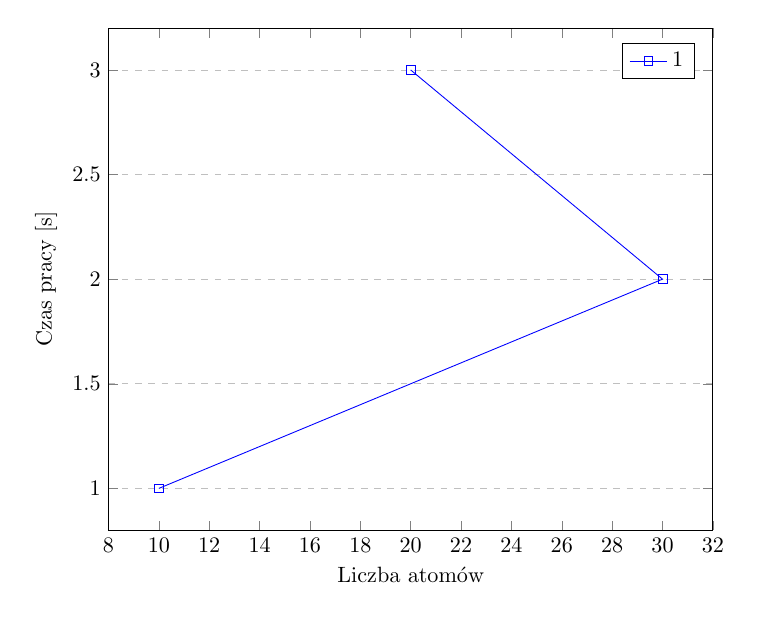
\begin{tikzpicture}[scale=0.8]
        \begin{axis}[
        xlabel={Liczba atomów},
        ylabel={Czas pracy [s]},
        %xmin=0,xmax=5500,
        %ymin=0,%ymax=0.0105,
        scale=1.4,
        legend pos=north east,
        ymajorgrids=true,grid style=dashed
        ]
        
        \addplot[color=blue,mark=square]
        coordinates {
            (10, 1)
            (30, 2)
            (20, 3)
        };
        \legend{1}
        \end{axis}
    \end{tikzpicture}
\end{center}

\begin{center}
    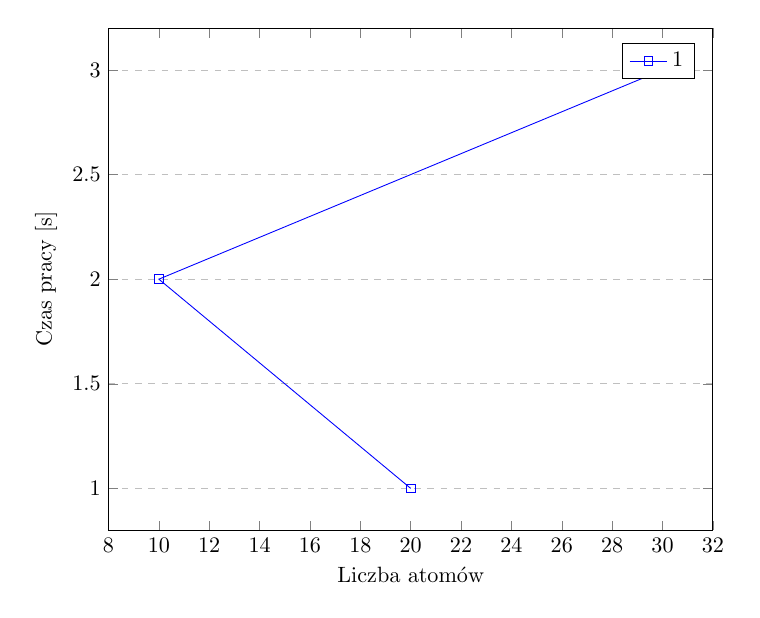
\begin{tikzpicture}[scale=0.8]
        \begin{axis}[
        xlabel={Liczba atomów},
        ylabel={Czas pracy [s]},
        %xmin=0,xmax=5500,
        %ymin=0,%ymax=0.0105,
        scale=1.4,
        legend pos=north east,
        ymajorgrids=true,grid style=dashed
        ]
        
        \addplot[color=blue,mark=square]
        coordinates {
            (30, 3)
            (10, 2)
            (20, 1)
        };
        \legend{1}
        \end{axis}
    \end{tikzpicture}
\end{center}

\end{document}
